\section{System Design}


\subsection{Use Cases}

\subsubsection{Use Case Actors}
The main actor that can be considered in this system is the \textit{user}, since no administrative accounts are available, nor are they considered necessary.
\begin{itemize}
  \item User
  \begin{itemize}
    \item Responsibilities in the system
    \begin{itemize}
      \item -
    \end{itemize}
    \item Possibilities in the system
    \begin{itemize}
      \item Manage student groups 
      \item Create courses, quizes, questions.
      \item Generate random or predefined quizes
      \item Uploading of completed quizes
      \item Automatic marking of the scanned quizes
      \item Saving/printing of the generated quizes
    \end{itemize}
  \end{itemize}
\end{itemize}


\subsubsection{Use Case Diagram}
The use case diagram \ref{use_case_diagram} presented below, shows the main actions that can be performed by an user inside the application. There are six direct actions presented for this purpose. The first one and the last two, counting from top to bottom, represent the managing part of the application, which includes the courses, quizes and questions. They have been chosen as actions to be described here, because togethe they comprise a big part of the application's functionality. This managing method is similar to a simplistic file manager system. You can do the basic operations in each compartment: create, delete, rename and view. The next action is about \textit{student group} and \textit{students} managing. It was not grouped together with the previous actions, because it does not have a direct contact with them in the front-end designed for the users. It practically does the same operations upon the created instances. The \textit{generate quiz} action is one of the two most essential actions, that the QTK is heavily relying on. From the user's point of view it represents a button that is present in all of the quizes' view pages. It is used to generate ready to print quizes, devised for specific purposes, that the user has in mind. This action also covers the action of choosing the options for generating those particular quizes. The \textit{upload quiz} action, is the second most important action, that simply represents the uploading of the completed quizes' scans to the application. This upload though, chains to itself two other indirect actions, that occur immediately after it is finished. These are the \textit{process quiz} action, which as the name suggests, process the image that was uploaded, and the \textit{mark quiz} action, which use the data aquired from the processing to give a rating to that quiz's filling.

\begin{figure}[!ht]
\centering
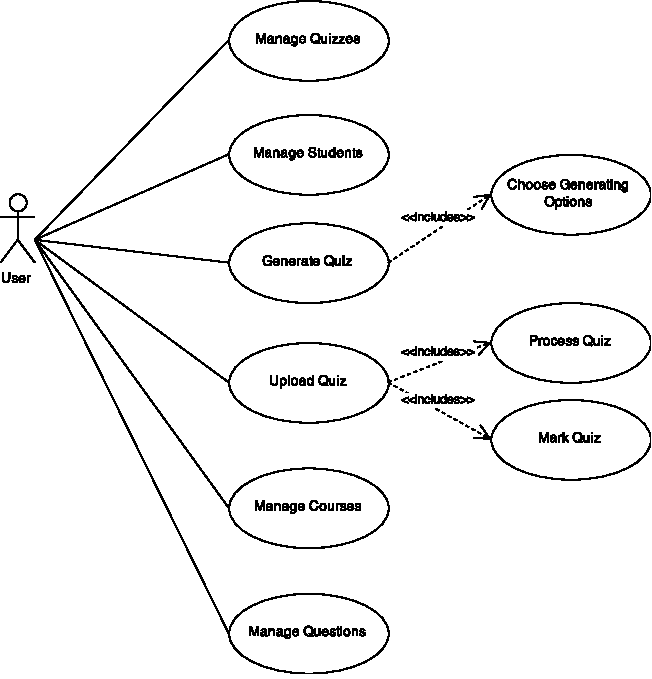
\includegraphics[scale=1.2]{use_case}
\caption{Use case diagram} \label{use_case_diagram}
\end{figure}

\subsubsection{Use Cases Description}
\begin{itemize}
  \item Register
  \begin{itemize}
    \item A teacher enters the system’s domain name in the browser
    \item A page appears, where the teacher clicks on the “Register” button
    \item The teacher is redirected to the register page
    \item He fills in the required fields and presses “Register”
    \item A message appears saying that an email has been sent to his address containing the confirmation link
    \item The teacher is redirected to the “Log in” page.
  \end{itemize}

  \item Log in 
  \begin{itemize}
    \item The user enters the system’s domain name in the browser. 
    \item A page appears, where the user must fill in his username and password and click the “Log in” button. 
    \item If authenticated successfully, the user will be redirected to his main page.
  \end{itemize}

  \item Create directories
  \begin{itemize}
    \item The user presses the “Create new” button, which is located above the directory list.
    \item A dialog window, that contains an input field  “Course name” and a button “Create”, appears.
    \item The user enters the name of  the directory and clicks “Create”
    \item This makes the dialog to vanish and the list to contain the new directory.
  \end{itemize}

  \item Delete directories
  \begin{itemize}
    \item The user marks the directories which are to be removed, by clicking on the box that is located to the left of the name of each directory. 
    \item Then he clicks on “Delete” button at the top of the list.
    \item A dialog appears, asking to confirm this action.
    \item The user clicks the “yes” button and the dialog disappears along with the chosen directories .
  \end{itemize}

  \item View a directory
  \begin{itemize}
    \item The user double-clicks the desired directory in the main page’s list
    \item The directory’s contents will appear instead of the courses list
  \end{itemize}  

  \item Create a quiz with manual input
  \begin{itemize}
    \item When user is in a course directory, he can create a new quiz
    \item He clicks the “Create new quiz” button
    \item A dialog  appears with two options: “Upload Quiz”, “Manual input”
    \item The user chooses the “Manual input”
  \end{itemize}

  \item Add question
  \begin{itemize}
    \item The user enters the question in the text area, presses the “Upload image” button to add an image to the question
    \item The user selects number of answers
    \item Fills in the answers
    \item Marks the correct answers
    \item Press “save” button
  \end{itemize}

  \item Create a tag
  \begin{itemize}
    \item When editing a question, the user presses “Add tag” button
    \item In the dialog, user writes in the text field the name of the tag
    \item User presses the “Create tag” button next to it
    \item The tag is created and it can be found in the dropdown list of the dialog
  \end{itemize}

  \item Add a tag to a question
  \begin{itemize}
    \item When editing a question, the user presses the “Add tag” button
    \item A dialog appears
    \item The user selects in the dropdown list the wanted tag
    \item The user clicks on the “Add tag” button
    \item The dialog disappears, and the tag is set
  \end{itemize}    

  \item Delete a quiz
  \begin{itemize}
    \item User selects from the list of quizes, the ones which should be deleted by checking the boxes.
    \item User clicks “delete” button
    \item User presses “yes” in the dialog window
    \item The selected quizes are deleted
  \end{itemize}    

  \item View a quiz
  \begin{itemize}
    \item User double-clicks a quiz from the course directory list
    \item The system shows all the questions of this quiz
  \end{itemize}    

  \item Edit a quiz
  \begin{itemize}
    \item When the user is in the quiz’s “view mode”, he can press the “edit” button near a question
    \item The question become editable
  \end{itemize}    

  \item Create a quiz with “upload” option
  \begin{itemize}
    \item The user clicks “create new quiz” button
    \item Presses “upload” button in the dialog window
    \item Then selects a file in the file manager window and presses “Upload”
    \item The quiz is created and the questions are created using the info in the file
  \end{itemize}

  \item Generate quiz
  \begin{itemize}
    \item In “view mode” of the quiz, the teacher presses “generate quiz” button
    \item A window with options appears
    \item The teacher selects the group for which the quiz is generated
    \item Checks the “random” option
    \item Presses “Generate”
    \item The new quiz file, containing all variants of the quiz is created in the course directory
  \end{itemize}

  \item Export quiz
  \begin{itemize}
    \item Teacher selects the generated file and presses the export button
    \item In the new dialog window, the teacher selects the destination directory
    \item Presses “Save”
    \item PDF file is saved on the machine
  \end{itemize}

  item Scan and process quizes
  \begin{itemize}
    \item The user clicks on “upload” button on the main page
    \item He selects the files and uploads them
    \item The system processes each file and get the necessary data from them
    \item The data is stored in the database
  \end{itemize}

  \item Create a student group
  \begin{itemize}
    \item The user clicks on the student group tab on the main page
    \item The system shows the list of groups and some buttons
    \item The user clicks on the create button
    \item The user is asked to enter the name of the group
    \item The user writes the name of the group and presses “Create”
    \item The new group appears in the list
  \end{itemize}

  \item Add a student to a student group
  \begin{itemize}
    \item The user double-clicks on a student group
    \item The system shows the list of students in that group
    \item The user presses on the “Add student” button
    \item He is prompted to enter the student’s name
    \item The user enters the name and clicks on “Add”
    \item The student appears in the list
  \end{itemize}
\end{itemize}

\subsection{Class Diagrams}

The diagram illustrated below, in figure \ref{controller_class}, represents the gathering of all the controller classes which describe the business logic of the QTK application. It is designed to show the actions that each of the classes have available and the hierarchy of inheritance. Every controller class inherits from ApplicationController, which in turn inherits from ActionController::Base. The core of a Rails application web requests are the Action Controllers. The actions that they consist of, are public methods which are executed on request. These methods are usually linked to a ``view'' template, that can be rendered as soon as the action is requested. They also can redirect to other methods. The controllers' actions are made available to the server by Rails Routes, which map URLs to these actions. 

\begin{figure}[!ht]
\centering
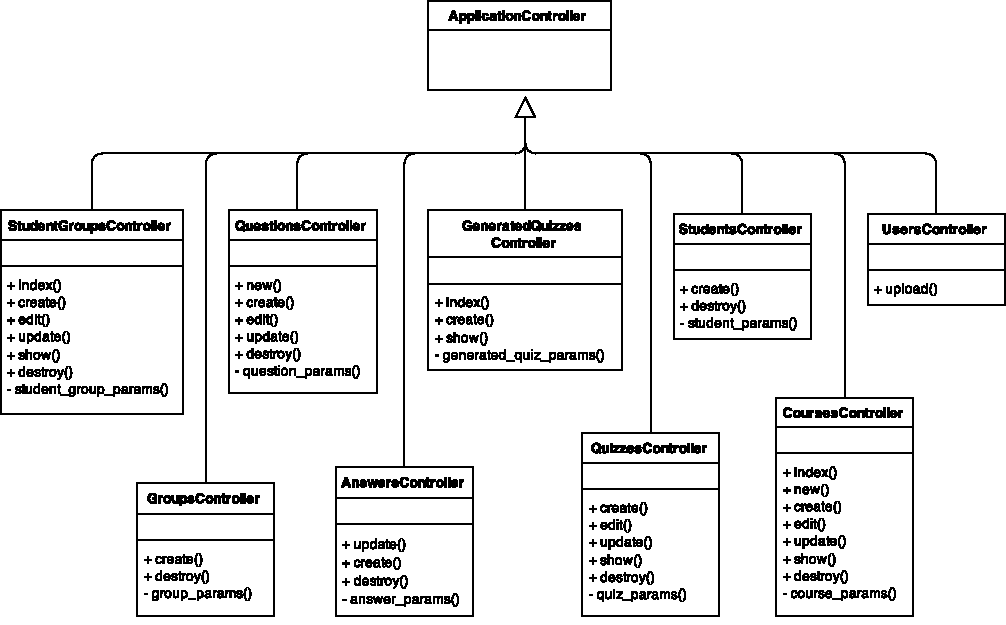
\includegraphics[width=\textwidth]{controller_class_dia}
\caption{Controller class diagram}\label{controller_class}
\end{figure}

The class diagram presented in figure \ref{model_class}, denotes the Model layer in the MVC pattern. It holds the model classes which represent, in an abstract way, the database tables. These classes inherit from the ActiveRecord::Base class. ActiveRecord is an ORM Framework which connect application objects to RDBMS tables. ActiveRecord gives the possibilty to indicate the relationship between these classes. Independent row instances that are extracted from the database will be objects of these classes type. Variables have been indicated in each class, to reflect the fields of the tables, that have the same name as these classes. Model classes record the associations between them, which is equivalent to the ones on the database level. These associations help manipulating the database in a object-oriented fashion, through ActiveRecord. Most of the associations between the model classes are one-to-many compositions. Only two of the relations are many-to-many associations, which do not have an intermediary class for the table that unites them. It can be observed that when the composition relationships are followed, the User class is at the end of the link. So, this means that when a user is deleted, most of the other instances related to it, will be also deleted. 

\begin{figure}[!ht]
\centering
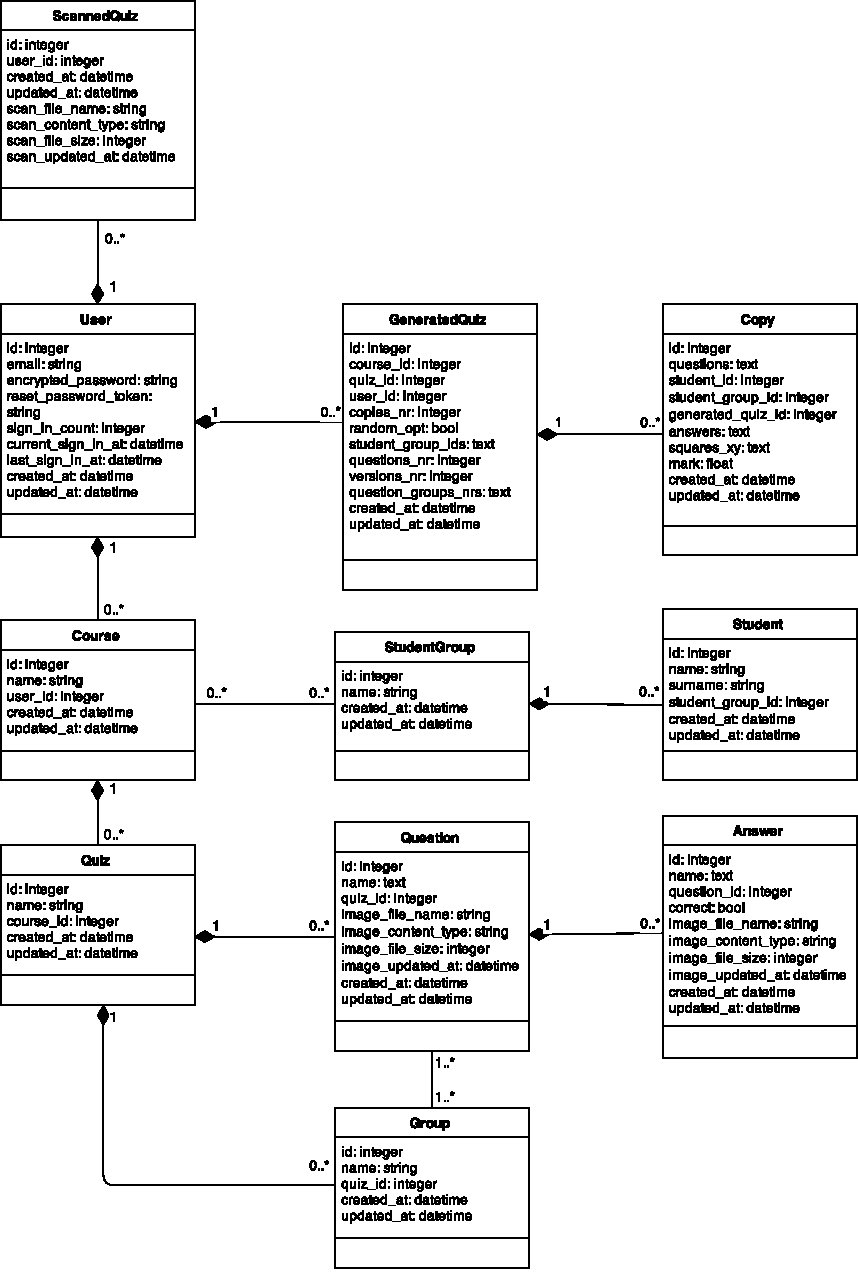
\includegraphics[scale=1]{class_diagram_model}
\caption{Model class diagram}\label{model_class}
\end{figure}

Since the processing of an image can take some time, it was necessary to make this as a separate process which runs in parallel. Thus, not making the web page to load for a indefinite amount of time when a bunch of images are being uploaded. The figure \ref{job_class}, which represents a class diagram of the classes related to background processing and image processing illustrates the relationship between them and the attributes and methods of the \textit{ScansProcessingJob} class. This class, or job is responsible for the uploaded images processing. Every method presented of the ScansProcessingJob, does a small part of the whole image processing. The \textit{perform} method is inherited from ActiveJob::Base and is a necessary part for the background processing to work. It utilizes and combines the other methods and integrate them into a single process, that evaluates uploaded images. 

ActiveJob is a framework that uses queueing backends to make the jobs run asynchronously. There are a variety of these backends that can be used with ActiveJob. That's why ActiveJob has adapters available for each of these queueing backends. So, to put the diagram into words, a class which is considered a job, inherits from ActiveJob::Base class, the needed adapter class is used(in this case is used a Resque adapter: ActiveJob::QueueAdapters::ResqueAdapter), which also inherits from ActiveJob::Base. Now, this adapter is directly associated with the Resque libary. This gives the possibility of changing the queueing backend whenever necessary, without having to change the class implementation, which depicts the job. 

\begin{figure}[!ht]
\centering
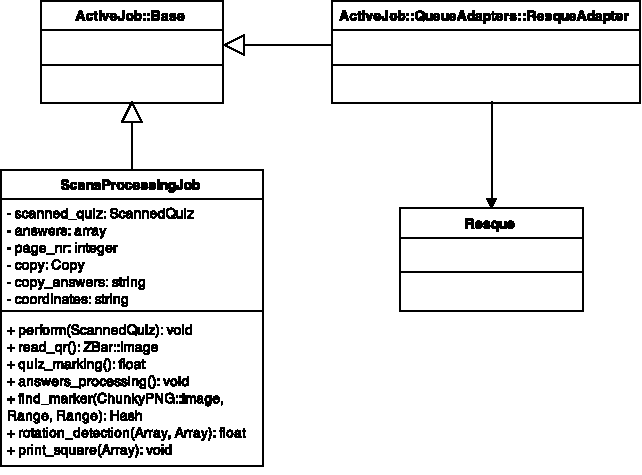
\includegraphics[scale=1.1]{background_job_class}
\caption{Background job class diagram}\label{job_class}
\end{figure}

The generation of the pdf file containing the quizes, is handled by the QuizPdf class presented in figure \ref{pdf_class}. QuizPdf inherits from Prawn::Document class, which is a class belonging to the Prawn library(a pure Ruby pdf generation library). In this simple class diagram, it is shown the private attributes and the public methods of the QuizPdf class. The acquaintance and usage of the Prawn API was essential in the implementation of the quiz generation fragment of the thesis.

\begin{figure}[!ht]
\centering
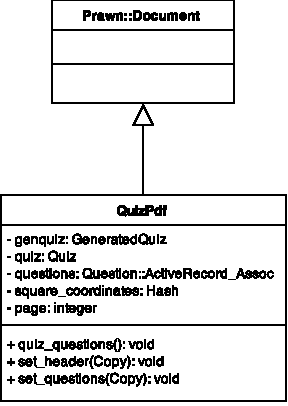
\includegraphics[scale=1]{pdf_generator_class}
\caption{Pdf generator class}\label{pdf_class}
\end{figure}

\subsection{Sequence Diagrams}
The flow of logic of quiz generation and quiz uploading/processing will be introduced in figures \ref{generate_sequence} and \ref{upload_sequence}. The diagrams will be covered step by step, being guided by the sequence of the messages. The entities that interact with each other in the diagram are enumerated:
\begin{enumerate} 
  \item User
  \item Application
  \item GeneratedQuizzesController class
  \item GeneratedQuizzesHelper class
  \item Copy class
  \item Database
  \item QuizPdf class
\end{enumerate}

The logic behind the quiz's generation starts with the \textit{user} begining the generation process, by completing the necessary generation options in the application's web interface and submitting it to the server. The application's server identifies this request as a \textit{create} controller action belonging to GeneratedQuizzesController class, using Rails Routes. The create action is called and the options which denote the type of generation to be performed, are passed along. Inside the GenerateQuizzesController class create action, the method \textit{gen\_copies} of the helper module GeneratedQuizzesHelper will be called. This method contains the logic behind creating the necessary Copy class instances, based on the options selected by the user when generating quizzes. Based on the amount of copies to be created, the method has an iterative procedure of creating Copy instances, and saving them to the database. After the method finishes its execution, the pdf generation process is triggered, by instatiating a new QuizPdf object. When the pdf is ready, it is assigned to a variable in the ongoing action. This variable, containing the pdf file is then sent to the user and rendered in the browser. The user can now save the pdf file and print it.

The second diagram has the following entities, that are fundamental for the quiz uploading process:
\begin{enumerate}
  \item User
  \item Application
  \item UsersController
  \item ScannedQuiz class
  \item Database
  \item Worker
  \item ScansProcessingJob class
\end{enumerate}

The process starts when the user uploads a set of image files through the application's web interface. The UsersController's upload action is commenced. Now, the upload action creates the ScannedQuiz instance for an image, which in its turn accesses the database and saves its image data. This is looped over, until all of the images are stored in the database. After ScannedQuiz instance is commited to the database, the ScansProcessingJob's \textit{perform\_later} method is called, providing the ScannedQuiz instance as argument. This method puts the argument data in a queue, that is going to be performed asynchronously. At the same time, a worker instance, which checks for jobs in the existent queues, every 5 seconds, needs to accesses them in the ScansProcessingJob class for the job. If a job is present, it is assigned to the worker that was the first to query for one. The worker performs the job and saves the results to the database in the process. When the job is finished, the worker queries for another one.

\begin{sidewaysfigure}[!ht]
\centering
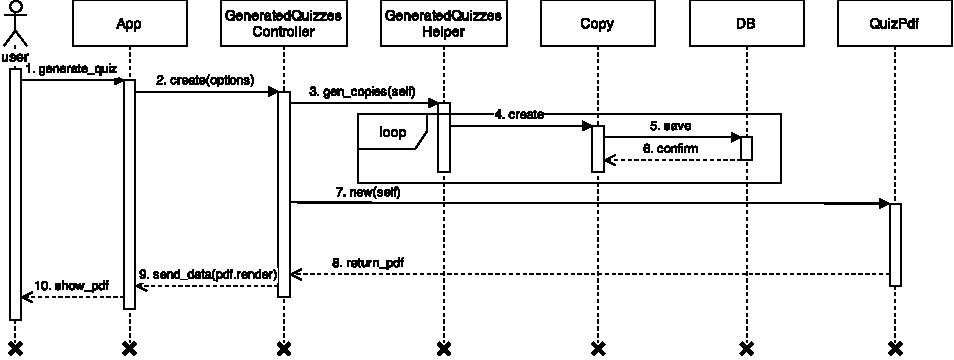
\includegraphics[scale=1.5]{generate_quiz_sequence}
\caption{Quiz generating sequence diagram}\label{generate_sequence}
\end{sidewaysfigure}

\begin{sidewaysfigure}[!ht]
\centering
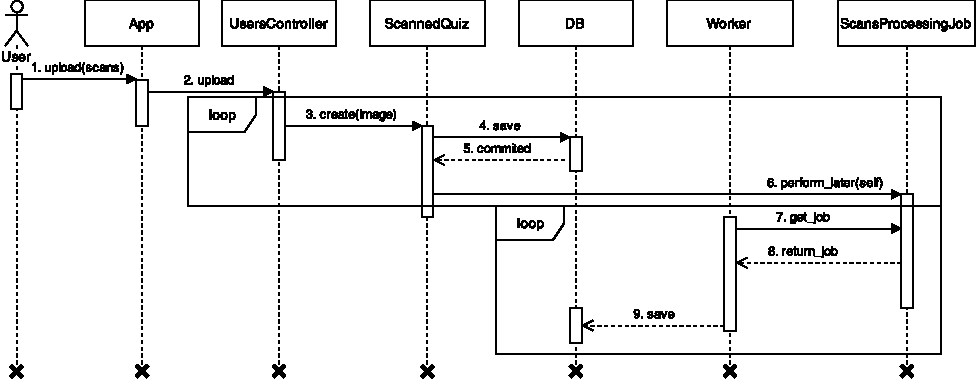
\includegraphics[scale=1.5]{upload_quiz_sequence}
\caption{Quiz uploading sequence diagram}\label{upload_sequence}
\end{sidewaysfigure}


\subsection{Activity and State Diagrams}
The activity and state diagrams will be used to present the processes: quiz generation\ref{generation_state} and quiz processing\ref{processing_activity}. Another aproach of visualizing these processes was performed, so that more perspective is added to the processes' analysis. 

The quiz generation state diagram shows the different states the application's web interface is in, at different stages of the attempt to generate a quiz. The user does a sequence of actions, which takes him from the main page of the app, to the rendered pdf file. Down this course of actions, the user finds the app's web interface in certain states, which correspond to the actions made.

The activity diagram takes the quiz processing through a list of activities and decision points. A begining state and final state is present. The diagram is designed to be in the system's point of view. It goes through processing the QR code, marker processing, marking of the test and persisting data to the database.

\begin{figure}[!ht]
\centering
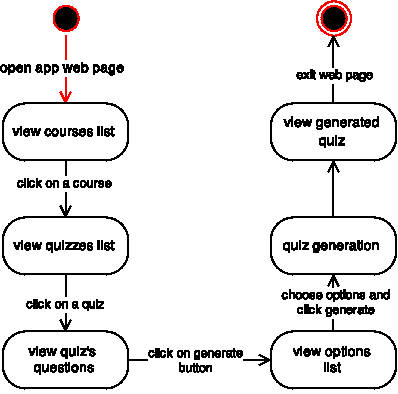
\includegraphics[scale=1]{generate_quiz_state_dia}
\caption{Quiz generation state diagram}\label{generation_state}
\end{figure}

\begin{figure}[!ht]
\centering
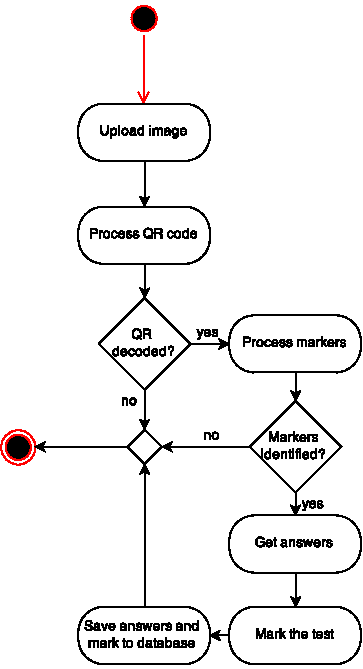
\includegraphics[scale=1]{uml_quiz_processing_activity}
\caption{Quiz processing activity diagram}\label{processing_activity}
\end{figure}







